\documentclass[journal,12pt,twocolumn]{IEEEtran}
\usepackage{setspace}
\usepackage{gensymb}
\singlespacing
\usepackage[cmex10]{amsmath}

\usepackage{amsthm}
\usepackage{hyperref}
\hypersetup{
    colorlinks=true,
    linkcolor=blue,
    filecolor=magenta,      
    urlcolor=cyan,
}

\urlstyle{same}
\usepackage{mathrsfs}
\usepackage{txfonts}
\usepackage{stfloats}
\usepackage{bm}
\usepackage{cite}
\usepackage{cases}
\usepackage{subfig}

\usepackage{longtable}
\usepackage{multirow}

\usepackage{enumitem}
\usepackage{mathtools}
\usepackage{steinmetz}
\usepackage{tikz}
\usepackage{circuitikz}
\usepackage{verbatim}
\usepackage{tfrupee}
\usepackage[breaklinks=true]{hyperref}
\usepackage{graphicx}
\usepackage{tkz-euclide}

\usetikzlibrary{calc,math}
\usepackage{listings}
    \usepackage{color}                                            %%
    \usepackage{array}                                            %%
    \usepackage{longtable}                                        %%
    \usepackage{calc}                                             %%
    \usepackage{multirow}                                         %%
    \usepackage{hhline}                                           %%
    \usepackage{ifthen}                                           %%
    \usepackage{lscape}     
\usepackage{multicol}
\usepackage{chngcntr}
\usepackage{mdframed}
\DeclareMathOperator*{\Res}{Res}

\renewcommand\thesection{\arabic{section}}
\renewcommand\thesubsection{\thesection.\arabic{subsection}}
\renewcommand\thesubsubsection{\thesubsection.\arabic{subsubsection}}

\renewcommand\thesectiondis{\arabic{section}}
\renewcommand\thesubsectiondis{\thesectiondis.\arabic{subsection}}
\renewcommand\thesubsubsectiondis{\thesubsectiondis.\arabic{subsubsection}}


\hyphenation{op-tical net-works semi-conduc-tor}
\def\inputGnumericTable{}                                 %%

\lstset{
%language=C,
frame=single, 
breaklines=true,
columns=fullflexible
}

\usepackage{chngcntr}
\counterwithin{figure}{section}

\title{AI5002}
\author{TUHIN DUTTA}
\date{January 2021}

\begin{document}
\newtheorem{theorem}{Theorem}[section]
\newtheorem{problem}{Problem}
\newtheorem{proposition}{Proposition}[section]
\newtheorem{lemma}{Lemma}[section]
\newtheorem{corollary}[theorem]{Corollary}
\newtheorem{example}{Example}[section]
\newtheorem{definition}[problem]{Definition}

\newcommand{\BEQA}{\begin{eqnarray}}
\newcommand{\EEQA}{\end{eqnarray}}
\newcommand{\define}{\stackrel{\triangle}{=}}
\bibliographystyle{IEEEtran}
\raggedbottom
\setlength{\parindent}{0pt}
\providecommand{\mbf}{\mathbf}
\providecommand{\pr}[1]{\ensuremath{\Pr\left(#1\right)}}
\providecommand{\qfunc}[1]{\ensuremath{Q\left(#1\right)}}
\providecommand{\sbrak}[1]{\ensuremath{{}\left[#1\right]}}
\providecommand{\lsbrak}[1]{\ensuremath{{}\left[#1\right.}}
\providecommand{\rsbrak}[1]{\ensuremath{{}\left.#1\right]}}
\providecommand{\brak}[1]{\ensuremath{\left(#1\right)}}
\providecommand{\lbrak}[1]{\ensuremath{\left(#1\right.}}
\providecommand{\rbrak}[1]{\ensuremath{\left.#1\right)}}
\providecommand{\cbrak}[1]{\ensuremath{\left\{#1\right\}}}
\providecommand{\lcbrak}[1]{\ensuremath{\left\{#1\right.}}
\providecommand{\rcbrak}[1]{\ensuremath{\left.#1\right\}}}
\theoremstyle{remark}
\newtheorem{rem}{Remark}
\newcommand{\sgn}{\mathop{\mathrm{sgn}}}

\providecommand{\res}[1]{\Res\displaylimits_{#1}} 

%\providecommand{\norm}[1]{\lVert#1\rVert}
\providecommand{\mtx}[1]{\mathbf{#1}}
\providecommand{\fourier}{\overset{\mathcal{F}}{ \rightleftharpoons}}
%\providecommand{\hilbert}{\overset{\mathcal{H}}{ \rightleftharpoons}}
\providecommand{\system}{\overset{\mathcal{H}}{ \longleftrightarrow}}
	%\newcommand{\solution}[2]{\textbf{Solution:}{#1}}
\newcommand{\solution}{\noindent \textbf{Solution: }}
\newcommand{\cosec}{\,\text{cosec}\,}
\providecommand{\dec}[2]{\ensuremath{\overset{#1}{\underset{#2}{\gtrless}}}}
\newcommand{\myvec}[1]{\ensuremath{\begin{pmatrix}#1\end{pmatrix}}}
\newcommand{\mydet}[1]{\ensuremath{\begin{vmatrix}#1\end{vmatrix}}}
\numberwithin{equation}{subsection}
\makeatletter
\@addtoreset{figure}{problem}
\makeatother
\let\StandardTheFigure\thefigure
\let\vec\mathbf
\renewcommand{\thefigure}{\theproblem}
\def\putbox#1#2#3{\makebox[0in][l]{\makebox[#1][l]{}\raisebox{\baselineskip}[0in][0in]{\raisebox{#2}[0in][0in]{#3}}}}
     \def\rightbox#1{\makebox[0in][r]{#1}}
     \def\centbox#1{\makebox[0in]{#1}}
     \def\topbox#1{\raisebox{-\baselineskip}[0in][0in]{#1}}
     \def\midbox#1{\raisebox{-0.5\baselineskip}[0in][0in]{#1}}
\vspace{3cm}
\title{AI5002 - Assignment 5}
\author{Tuhin Dutta\\ ai21mtech02002}
\maketitle
\newpage
\bigskip
\renewcommand{\thefigure}{\theenumi}
\renewcommand{\thetable}{\theenumi}
\begin{mdframed}
Download code and LaTeX from below hyperlinks\\
1. \href{https://github.com/Tauhait/AI5002/blob/main/Assignment-5/Codes/MiscellaneousDistributions\_5\_31.py}{Codes/MiscellaneousDistributions\_5\_31.py}


2. \href{https://github.com/Tauhait/AI5002/tree/main/Assignment-5/LaTeX}{LaTeX}
\end{mdframed}
\subsection*{\boldsymbol{Problem\ 5.31}}
\begin{flushleft}Two cards are drawn simultaneously (or
successively without replacement) from a well
shuffled pack of 52 cards. Find the mean,
variance and standard deviation of the number
of kings.\end{flushleft}

\subsection*{\boldsymbol{Solution}}\\
\begin{flushleft}Let X be a random variable.\newline
X = Number of kings present in the two cards drawn from a well shuffled pack of 52 cards.\newline
\newline The values that X can have are = \Big\{ 0, 1, 2 \Big\}.\\
\newline The probability of X taking each of the above values are - \end{flushleft}
\begin{align}P(X=0) = \dfrac{\binom{48}{2}}{\binom{52}{2}} = \dfrac{188}{221} \approx 0.8507\end{align}
\begin{align}P(X=1) = \dfrac{\binom{4}{1} * \binom{48}{1}}{\binom{52}{2}} = \dfrac{32}{221} \approx 0.1448\end{align}
\begin{align}P(X=2) = \dfrac{\binom{4}{2}}{\binom{52}{2}} = \dfrac{1}{221} \approx 0.0045\end{align}
\newline
\begin{flushleft}The Mean calculated as E(X) is given by,\end{flushleft}
\begin{align}E(X) = \sum X.P(X) \end{align}
\begin{align*}= 0*\dfrac{188}{221} + 1*\dfrac{32}{221} + 2*\dfrac{1}{221}\end{align*}
\begin{align*}= \dfrac{34}{221} \approx 0.154\end{align*}
\begin{align*}E(\mathop{X^2}) = \sum \mathop{X^2}.P(X)\end{align*}
\begin{align*}= 0^2 * \dfrac{188}{221} + 1^2 * \dfrac{32}{221} + 2^2 * \dfrac{1}{221} = \dfrac{36}{221}\end{align*}
\newline
\begin{flushleft}The Variance calculated as Var(X)is given by,\end{flushleft}
\begin{align}Var(X) = E(\mathop{X^2}) - \mathop{[E(X)]^2}\end{align}
\begin{align*} = \dfrac{36}{221} - \mathop{\Bigg[\dfrac{34}{221}\Bigg]^2} = \dfrac{6800}{48841} \approx 0.139\end{align*}
\newline
\begin{flushleft}The Standard-Deviation calculated as SD(X) is given by,\end{flushleft}
\begin{align}SD(X) = \sqrt{Var(X)} = \sqrt{0.139} \approx 0.373\end{align}
\begin{figure}[h!]
    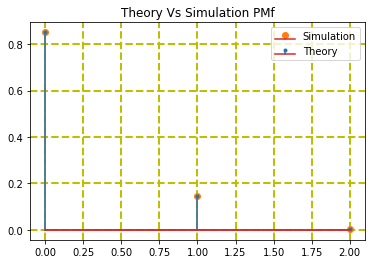
\includegraphics[width=15cm]{Assignment-5/Codes/Figures/theoryVsSimul_pmf.png}
    \caption*{Fig 1.1: Theory Vs Simulation of PMf}
\end{figure}
\begin{figure}[h!]
    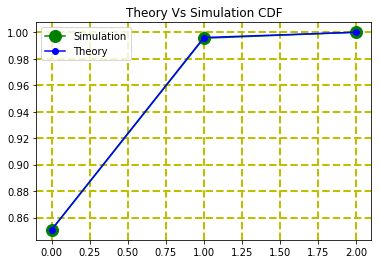
\includegraphics[width=15cm]{Assignment-5/Codes/Figures/theoryVsSimul_cdf.png}
    \caption*{Fig 1.2: Theory Vs Simulation CDF}
\end{figure}
\end{document}
